% Mandatory document setup
\documentclass[11pt]{article}
\usepackage[a4paper]{geometry}

% Default formatting packages
\usepackage{booktabs}
\usepackage{graphicx}
\usepackage{pdflscape}            
\usepackage{afterpage}
\usepackage{caption} 
\captionsetup{font=small,labelfont={bf},width=0.95\textwidth} % smaller caption font size
\usepackage{subcaption}

% Extra formatting packages
% \usepackage{setspace}
\usepackage{gensymb}
% \usepackage{multirow}
% \usepacakge{multicolumn}
% \usepackage{hyperref}
% \hypersetup{colorlinks=false, pdfborder={0 0 0}}

% Math fonts and extra environments for formulas
% \usepackage{amsmath}
% \usepackage{mathtools}
% \usepackage{textcomp}

% Citation formats and processors
\usepackage[style=apa, backend=biber]{biblatex}
\addbibresource{bib.bib}

% Internal references, this MUST be the last package loaded.
\usepackage{cleveref}

\frenchspacing

\title{Tectonics of the Reno River Basin}
\author{Jochen Wuttke}
\date{\today}

\begin{document}
\maketitle

\section{Introduction}

The Northern Apennines are a mountain range that sits on the asymmetrical orogenic wedge 
of the subduction zone between the overriding Tyrrhenian and the subducting Adriatic plate.
The subducting Adriatic plate is retreating towards the east, and the Tyrrhenian plate
shows extension in the Ligurian sea.
While the shortening in the east-facing pro-wedge is normal accretion from subduction,
the rollback of the Adriatic slab and the entire subduction zone causes the extension
in the interior of the orogen, concentrated on the retro wedge \parencite{erlanger-2020}.
The Apennines represent one of the best exposed and studied orogens of this type where
a retreating subduction zone influences the development of the accretionary orogen \parencite{picotti-2008}.

The topography of the mountain belt is asymmetrical, and while normal faults reach the surface 
in the extension zone of the retro-wedge, the mountain front shows no reverse faults that
could accommodate the shortening necessary for the observed uplift rates. 
River terraces provide evidence of ongoing uplift at least since then Pleistocene,
and earthquake activity supports the interpretation that the mountain front is still
actively deforming \parencite{picotti-2008}.
Rivers as the agents of transport integrate uplift and erosion, thus studying river profiles,
sediment flux and river terraces can provide insight into the tectonic dynamics of the orogen.

This report focusses on interpreting the river profiles of the main and tributary channels
in the Reno basin combined with the elevation and extent of river terraces in the lower basin
to model and constrain uplift and erosion rates in the Northern Apennines since the Pleistocene.
Additionally, the terraces above the surface and the corresponding sedimentary layers below the
surface in the Po plain are used to model the shape, size and depth of a hypothesized blind
thrust fault that could provide the observed uplift and deformation rates.

\section{Background}

The orogenic wedge as it is exposed on the surface today was constructed over the past 30 Ma.
Throughout that time, it was capped by a unit of ophiolites (Ligurian unit, \cref{fig:lithologies})
that passively rode on top of the wedge, and was covered by shallow marine sediments~(Epiligurian unit).
The wedge was partially built and uplifted through underplating with deep marine sediments from the
trench and deeper crust \parencite{picotti-2008}. The shallow-angled pro-wedge exposes all
three units in places, while the steeper angled retro-wedge exposes only the deep marine turbidites
in our study area that stretches towards the southwest starting from Bologna in \cref{fig:lithologies}.
Northeast of the mountain front lies the Po plain, the geomorphic expression of a completely 
sediment-filled basin.

\begin{figure}
    \centering
    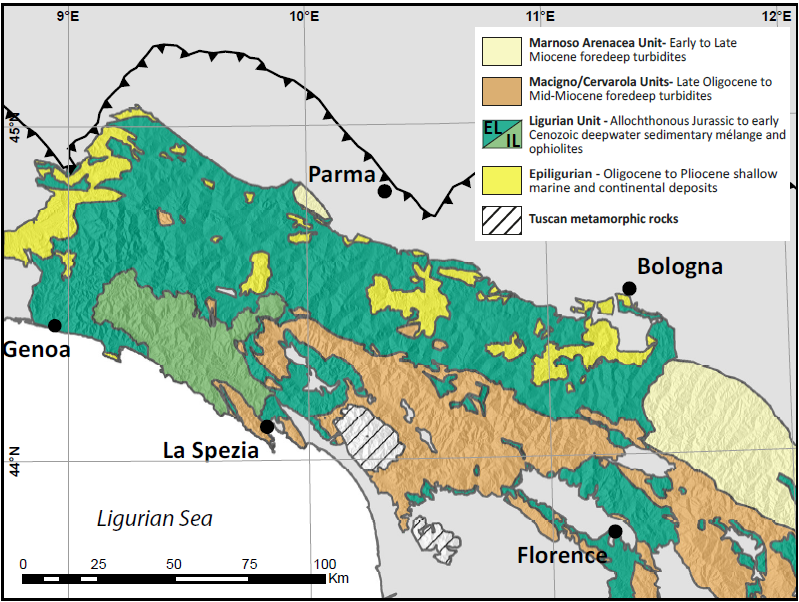
\includegraphics[width=0.95\textwidth]{lithologies.png}
    \caption{Main lithologies found in the Northern Apennines. These directly correspond to
    their tectonic origins: the Ligurian ophiolites stem from the ocean floor of the Ligurian sea, 
    later covered by the Epiligurian shallow marine sediments in some basins. The deep marine 
    turbidites of Macigno/Cervarola units underplate the wedge and Ligurian lid \parencite{picotti-2008}.
    Figure from \textcite{erlanger-2020}.}\label{fig:lithologies}
\end{figure}

The river valleys on the pro-wedge side expose several generations of strath terraces, reaching back in time
at least until the mid-Pleistocene. Strath terraces form when the river valley widens during times of relatively 
high sediment load and low total discharge of the river.
Wide, very shallow-angled flat areas on the river banks are eroded at those times, and covered with a usually
thin layer of alluvial debris. Multiple terraces document a continuing history of uplift and changing 
bed load and discharge conditions. When reliably dated, uplift rates and climate conditions at the time of 
their formation can be estimated \parencite{burbank-anderson-2nd-2016}.

\section{Methods}

To understand the tectonic history of the Northern Apennines and to infer the current
tectonic activity in the region, we analysed a number of geological key features and markers.

The overall shape of the orogen, the position of the main drainage divide and the shape and size 
of the Reno river basin were derived from a high resolution DEM and the topographic map of the region.
Hack's Law \parencite{hack1957studies} connects stream length $L$ and drainage area $A$, or respectively
the slope profile $S$ and drainage area with, importantly, empirical constants that
describe the general erosional behaviour of the drainage basin:
\begin{equation}
    L = k_aA^h
\end{equation}
\begin{equation}
    S = k_sA^{-\theta}
\end{equation}
Where L, S, and A are measured from maps and DEMS, and $k_a$, $h$, $k_S$ and $\theta$ are empirical constants
can be derived from regression over the log-log representation of the corresponding L/A and S/A plots.
These constants were used for further modelling in the common stream power river incision model (e.g. \textcite{burbank-anderson-2nd-2016})
\begin{equation}
    E = KA^mS^n
\end{equation} 

The model states that erosion $E$ is a function of the area $A$ of the drainage basin and the steepness $S$ of
the river. $K$ subsumes all other empirical constants and is commonly referred to as erodibility, while $m$ and $n$
control the relative importance of catchment area and steepness to overall erosion.

Assuming a steady state between erosion and uplift \parencite{whipple-1999} and substituting $S$ and $A$
with expressions from Hack's law, a multi-parameter
model to estimate erosion and uplift for river sections between knickpoints was obtained. Only uplift $U$, 
erodibility $K$ and the parameter $m$, roughly indicating whether erosion is proportional to total stream power
or specific stream power \parencite{burbank-anderson-2nd-2016}, were parameters to fit the model curves to the profile.

Detailed knickpoint analysis of the Reno main channel and several tributary channels related the identified
knickpoints to lithological and topographic boundaries in the basin, where possible.
Whether these are transient or stationary knickpoints gives important information about the tectonic
activity in the basin.

Borehole and seismic data were used to connect the sedimentary layers in the Po basin with the terraces
in the Reno river basin. The terraces are interpreted to show tectonic uplift rates \parencite{burbank-anderson-2nd-2016},
and trishear modelling \parencite{erslev_trishear_1991} was used to determine 
the direction and slip of the tectonic fault causing the uplift and deformation of the mountain front.

The terrace size and elevation used in several of the modelling steps was collected during a week-long field campaign
in May 2026 and combined with older data from \textcite{picotti-2008}.

\section{Results}

The topography of the northern Apennines is defined by two parallel mountain ridges running NW to SE (\cref{fig:topo}). 
The more eastern ridge is the high point of the entire mountain range and defines the main drainage divide.
Across the range from north to south, the slopes get steeper east to west, getting very 
steep close to the high points of both mountain ridges (\cref{fig:swaths}). Both the valley separating the ridges
and the mountain slopes on the western side are much steeper than in the east. 
This is particularly pronounced in southern part (\cref{fig:swath2}).

% The land surface in the Reno basin is flat and terraced compared to the surrounding and more upstream valleys (\cref{fig:reno}).
% The locally lowest terrace/surface area is defined by the stream bed and the terraces increase in elevation
% from the streambed outwards up the slopes. In the center of the valley, human construction is obscuring the
% elevation patterns somewhat, and at the sides of the valley, tributary streams have eroded some of
% the terraces.

\begin{figure}[b!]
    \centering
    \includegraphics[width=0.9\textwidth]{../HW01/NA_topo.png}
    \caption{Topographic map of the Northern Apennines. The elevation and slope profiles of the swaths 
    marked in blue are shown in \cref{fig:swaths}.}\label{fig:topo}
\end{figure}
    
\begin{figure}
    \centering
    \begin{subcaptionblock}{0.45\textwidth}
    \centering
    \includegraphics[width=\textwidth]{../HW01/swath_slopes_1.png}
    \caption{Northern swath.}\label{fig:swath1}
    \end{subcaptionblock}\qquad
    \begin{subcaptionblock}{0.45\textwidth}
    \centering
    \includegraphics[width=\textwidth]{../HW01/swath_slopes_2.png}
    \caption{Southern swath.}\label{fig:swath2}
    \end{subcaptionblock}
    \caption{Elevation and slope profiles across the Apennines. Blue arrows indicate the trends in \emph{slope} not elevation.
    Note that subfigures
        \subref{fig:swath1} and \subref{fig:swath2} have different $x$- and  $y$-axis scales.}\label{fig:swaths}
\end{figure}

The terrace location and elevation we collected in the field campaign, combined with the  downstream terraces from 
\textcite{picotti-2008}, are shown in \cref{fig:river_profile}.
Using age data, also from \textcite{picotti-2008}, the elevation difference maps to the uplift/incision rate estimates
shown in \cref{fig:incision_error}.
Uplift rates varied significantly between 0.5-2mm/yr over time only in the Pleistocene. The red and orange terraces
indicate uplift rates similar to the uplift measured from GPS stations, while younger terraces show
much higher uplift rates.
The younger uplift rates also show three distinct local minima, which coincide with steps in
the current Reno river (\cref{fig:uplift_relative}). These sharp dips in calculated uplift and the steps
in the river profile suggest that these are dams in the river. At the dam, the river is seemingly higher than
elsewhere, leading to low calculated uplift rates. After the dam the river immediately drops to its normal profile,
and thus a consistent uplift rate with the rest of the profile. Above the dam, the transition takes longer, leading
to a shallower incline in the uplift curve, until the "lake" built by the dam transitions back into the normal river profile.
The effect is strongest with the younger terraces, that show the least total uplift (not uplift rate).
These dams are most likely located at natural knickpoints, because the river gradient there is steeper, requiring shorter
canals to utilize the water power from the dams. These knickpoint are not associated with the faults shown in \cref{fig:knickpoint_map},
the terraces are all in the lower basin, the mapped faults are all in the upper basin. However, it is possible that faults
exist there, given that this is part of the compression zone of the accretionary wedge.

% This suggests that these knickpoints are the result of faults, and those 
% faults possibly activated \emph{after} the red and orange terraces formed. Due to the age and 
% considerable diffusion changes of the old terraces, it is also possible that the knickpoints
% exist but are not visible in the sparse data available.
% The thrust faults seem to uplift from left to right in the plots, which is westward (upriver)
% in the measurement data. 
% Interestingly, the errors for the estimated incision rates are higher for the younger terraces
% for the older terraces. Possibly because the plotted lines are smooth for the old terraces, and
% limited variance translates to low errors.

\begin{figure}
    \centering
    \begin{subcaptionblock}{0.45\textwidth}
        \centering        
        \includegraphics[width=\textwidth]{../HW03/river_profile_sec7.png}
        \caption{Smoothed river profile with terrace elevation data.}\label{fig:river_profile}
    \end{subcaptionblock}\qquad
    \begin{subcaptionblock}{0.45\textwidth}
        \centering        
        \includegraphics[width=\textwidth]{../HW03/incision_error.png}
        \caption{Incision rate and uncertainty estimated from the data in \subref{fig:river_profile}.}\label{fig:incision_error}
    \end{subcaptionblock}\qquad
    \caption{River terrace elevation and location along the main channel, and incision rates derived from elevation
    differences and estimated ages in \textcite{picotti-2008}.}
\end{figure}

\begin{figure}
    \centering
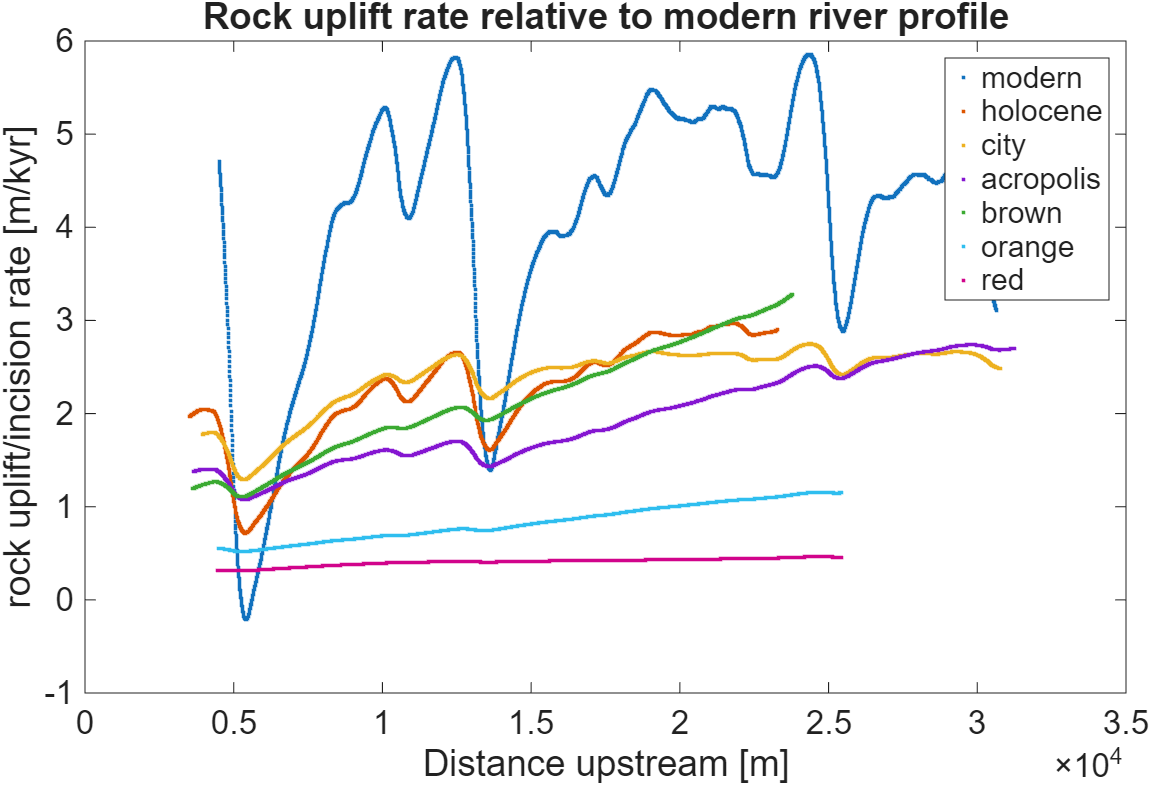
\includegraphics[width=0.45\textwidth]{uplift_relative.png}
\caption{Terrace uplift rates relative to modern river.}\label{fig:uplift_relative}
\end{figure}

The uplift estimates from \cref{fig:incision_error} were used to guide the fitting of the model parameters $K$ and $m$
in the stream power incision model (\cref{tab:data}).
First, using the area and slope information from the DEM, the regression parameters to Hack's Law, $k_a$ and $h$
were computed for the three river segments with a distinct slope profile each (cf. \cref{fig:area_plot}).
Similarly, the parameters $\theta$ and $k_s$ were estimated by regression over the slope-area plots for each segment.
Taking these values as constant, aiming for $U$ to be in the range of 2-3mm/yr, only $K$ and $m$ remain as free
variables to fit the model. It has to be noted that the middle segment has a convex profile instead
of the expected concave profile. That reduces the quality of the fit and makes some of the results of the 
regressions unusable. In those cases, the values from the similarly steep top segment were used.
The final result is shown in \cref{tab:data}. \Crefrange{fig:fit_top}{fig:fit_bottom} in the appendix show the
quality of the individual fits.

\begin{table}
    \centering
    \caption{Key data, measurements and estimated values for the river segments.
    The names ``top'', ``middle'', ``bottom'' refer to the segments with increasing 
    distance from the drainage divide. $\theta=0.77$ for the bottom segment 
    was outside the suggested valid range, so we used 0.65 for the fitting.
    The slope regression for the middle segment yielded a negative $\theta$, but the simulation
    can handle only positive values, so we used the absolute value.}\label{tab:data}
    \begin{tabular}{lrrr}
        \toprule
        & \textbf{Top} & \textbf{Middle} & \textbf{Bottom} \\\midrule
        Distance & 0-8\,km & 8-25\,km & 25-83\,km \\\midrule
        Slope regression &&&\\
        $k_s$ & 17.2 & 0 & 25544\\
        $\theta$ & 0.44 & -0.42 & 0.77 (0.65) \\\midrule
        Hack parameters &&& \\
        $k_a$ & 95732 & 253 & 16 \\
        $h$ & 0.55 & 1.3 & 1.6 \\\midrule
        U [mm/yr] & 2.3 & 3 & 2 \\
        K & $5\cdot 10^{-6}$ & $1.3\cdot 10^{-6}$  & $1\cdot 10^{-6}$\\
        \bottomrule
    \end{tabular}
\end{table}

\begin{figure}
    \centering
    \includegraphics[width=0.85\textwidth]{../HW04/area_plot.png}
    \caption{River elevation profile (left) and log-log slope-area plot of the Reno trunk channel.}\label{fig:area_plot}
\end{figure}

In \cref{fig:knickpoint_map} there are four distinguishable zones of differing river steepness in the basin.
Starting from the drainage divide, there is a narrow zone with only moderate steepness (black-blue).
In some places that zone is fairly clearly separated from the next steepness zone (green)
by knickpoints. But not all rivers show those knickpoints and the match isn't perfect anywhere.

The second zone is moderate to high steepness (green-orange). That zone is delineated downriver
by the lithological contact between the Macigno/Cervarola and Ligurian units. There is also
as fault. This change in steepness zones is also clearly marked by knickpoints in all the rivers
we analysed.

The third steepness zone stretches from the topmost fault almost to the mouth of the basin and
is predominantly shallow. Towards the mouth, the river slopes shallow even more. There are no
knickpoints for that final transition, and it is most likely the natural flattening of the basin, 
only visible as a sharp transition due to the way the steepness profile was coloured.

The first three zone transitions map well to the different slope profiles in \cref{fig:area_plot}. 
As mentioned, the last zone is likely an artifact of the data categorization, not a distinct
steepness zone.

Most of the identified knickpoints mark boundaries between the different steepness zones.
The knickpoints fall into three groups, clearly identifiable in \cref{fig:knickpoint_map}:
\begin{itemize}
    \item Points associated directly with faults.
    \item Points close to the divide, visible along the entire west-east stretch of the map.
    \item Few points in the Ligurian. They are not consistently identifiable in all streams, so
    may be due to local effects like landslides or dams.
\end{itemize}

\begin{figure}
    \centering
    \includegraphics[width=\textwidth]{../HW05/Map.png}
    \caption{Map showing the lithology, river steepness and knickpoints in the Reno basin.}\label{fig:knickpoint_map}
\end{figure}

Using the correlation of terraces and the alluvial subsurface stratigraphy before the mountain front 
provided by \textcite{picotti-2008}, a trishear model was fitted to the data of the oldest terraces
we encountered in our field campaign (Qt2-4). 
For simplicity, we kept the fault tip location relative to the mountain front constant at (10km/-15km), as well
as the propagation to slip ratio at 1.5. With the reduced scope of parameters, for each terrace/subsurface stratum
combination we fitted the model. For the younger terraces, finding a good fit proved difficult and is omitted here.
While no fit is perfect and no single set of fitting parameters
is sufficient to model all terraces, fitting parameters that work are all within the same rough area
of a dip angle of around -50\degree but with varying fault slip speeds (\cref{tab:trishear}).
\Crefrange{fig:fit_red}{fig:fit_brown} show the quality of the fitted curves.

\begin{table}
    \centering
    \caption{Fitted parameters in the trishear model. Negative dip means dip is towards the mountain. Model 
    parameters kept constant are the fault tip location and P/S ratio.}\label{tab:trishear}
    \begin{tabular}{lcc}\toprule
        \textbf{Terrace} & \textbf{Dip [\degree]} & \textbf{Slip velocity [mm/yr]} \\\midrule
        Qt2 (red) & -51 & 1\\
        Qt 3 (orange) & -50 & 1.9 \\
        Qt 4 (brown) & -49 & 4.5 \\\bottomrule
    \end{tabular}
\end{table}

\section{Discussion}

The topographic profiles in \cref{fig:swaths} recall the typical shape of a convergent orogen 
(\cref{fig:convergent_orogen}). In more detail, to the west, on the retro-wedge side, the deep valley
suggests extensional thinning of the wedge. In an accretionary wedge like this, we should expect
thrust faults towards the front of the pro-wedge, within the retro-wedge, and because we see
some evidence of extension, we should also see normal faults supporting that extension.
Published profiles in the literature suggest the thrust faults in both directions are present, and
at least in the retro-wedge reach the surface (e.g. fig. 8a in \textcite{picotti-2008}).
The extensional zone of the retro-wedge is not part of our study.

\begin{figure}
    \centering
    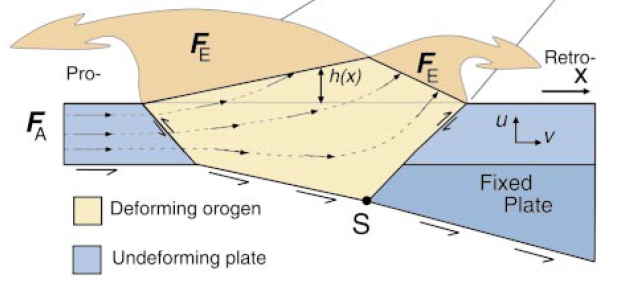
\includegraphics[width=.5\textwidth]{Accretionary-wedge-willet.png}
    \caption{Kinematic model of the accretionary wedge in a convergent orogen after \textcite{willett_steady_2002}.
    Material fluxes $F_A$ through accretion and $F_E$ by erosion define the shape of the orogen in steady state.}
    \label{fig:convergent_orogen}
\end{figure}

The river terraces document continuous uplift in recent history, suggesting that the  
mountain front is actively uplifting. Literature also documents earthquake belts that align with the expected
location of the faults \parencite{picotti-2008}. Trishear modelling of the mountain front and near-mountain part
of the Po plain is consistent with the presence of a deep blind thrust fault at an angle of roughly 50\degree, and
uplift rates around 1-2mm/yr. 

At the same time, the formation of the river terraces, especially the younger ones, documents changes in sediment
transport conditions. Those conditions have most likely been determined by climate changes rather than dramatic 
changes in uplift. Dry cold periods would support high sediment load, low discharge scenarios where the valley
would widen, and little to no vertical incision happens. In some cases, the ages of the terraces match up with
ice ages, but the younger terraces are all of Holocene age, so their genesis cannot be explained by ice ages.

The knickpoints of the Reno main channel and its tributaries (\cref{fig:knickpoint_map}) potentially document
features:
Some align with known faults, and thus are likely stationary knickpoints caused by the uplift at those faults. 
Some align with changes in lithology. This may also reflect a change in erodibility, and thus would cause a
stationary knickpoint.
Some few are not associated with either type of boundary. Because they are no present consistently in all
channels, they most likely are \emph{not} related to changes in uplift rate, but document local events
like landslides.

The data these interpretations are based on are naturally uncertain, e.g. dating the terraces based on soil formation
introduces some uncertainty beyond the pure uncertainty of the method itself. The derived uplift rates and
fault location and movement are all based on models that make simplifying assumptions, and additionally, we made 
further simplifying assumptions, like keeping specific model parameters constant to keep modelling effort manageable.
That leads to large uncertainties in the model results. Additionally, multi-parameter models usually allow
multiple best-fit solutions to given observed data. We used measured field data to drive the modelling efforts, 
e.g. we used the uplift rates derived from the terrace elevations today to fit stream slope curves matching that uplift.
However, that compounds the problem and ignores potential other, less rationally supported solutions. 

\section{Conclusion}

The data from our field campaign and the literature constrain geomorphic models of uplift and tectonics.
They consistently document continuous uplift throughout the Pleistocene, with uplift rates 
in modern times higher than those documented by the oldest terraces. Trishear modelling supports the
interpretation that this uplift is caused by a blind thrust fault. 
The basin stratigraphy derived from borehole data and modelling show that the Po basin is a km deep, 
sediment-filled basin ahead of the mountain front.
However, it is too far from the subduction trench to be directly related to it. 
The presence of the blind thrust fault suggests that the Po basin is a basin formed by the syncline of the
trishear deformation \parencite{erslev_trishear_1991}.

The recent GPS levelling data shows that the mountain front today is uplifting, and all modelling allows
for the observed uplift rates with sensible model parameters. The river terraces also support modern
uplift rates, and the hypothesized thrust fault provides much of the mechanism for this uplift.
It is possible that additional uplift is caused by underplating of the accretionary wedge, but that would 
lead to no observable geomorphic structures, and requires seismic studies and modelling to assess.

That the mountain front is actively uplifting, supported by an active fault provides an explanation for 
the observed seismicity of the region, and is probably the main source for it. This can inform
planning and development decisions in the region with expectations of regular strong seismicity.

% Referenced in a figure caption.
\nocite{capozzi_spontaneous_2010}
\printbibliography
\clearpage

\section*{Additional figures}

% River-slope model fits.
\begin{figure}[h]
    \centering
    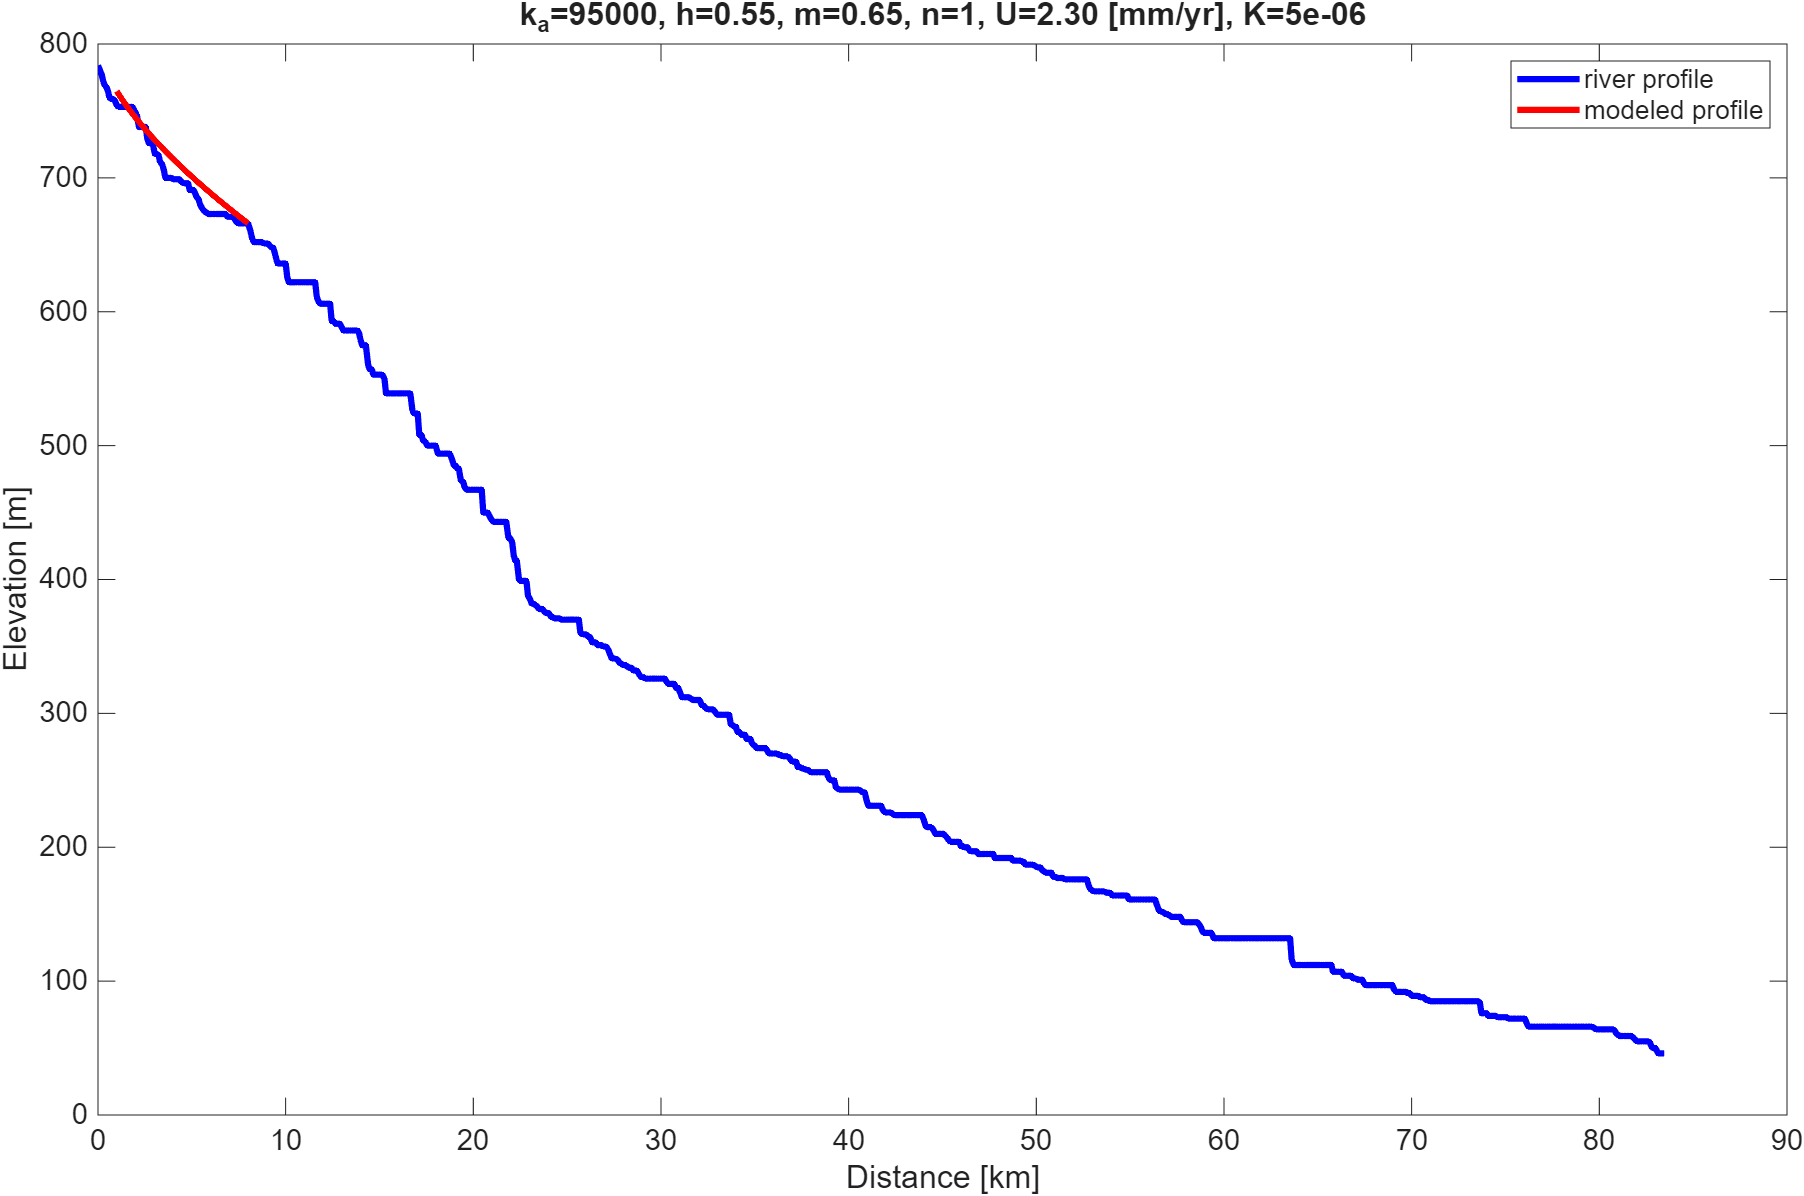
\includegraphics[width=0.8\textwidth]{fit_top_new.png}
    \caption{Fitted slope gradient, top section.}\label{fig:fit_top}
\end{figure}

\begin{figure}[h!]
    \centering
    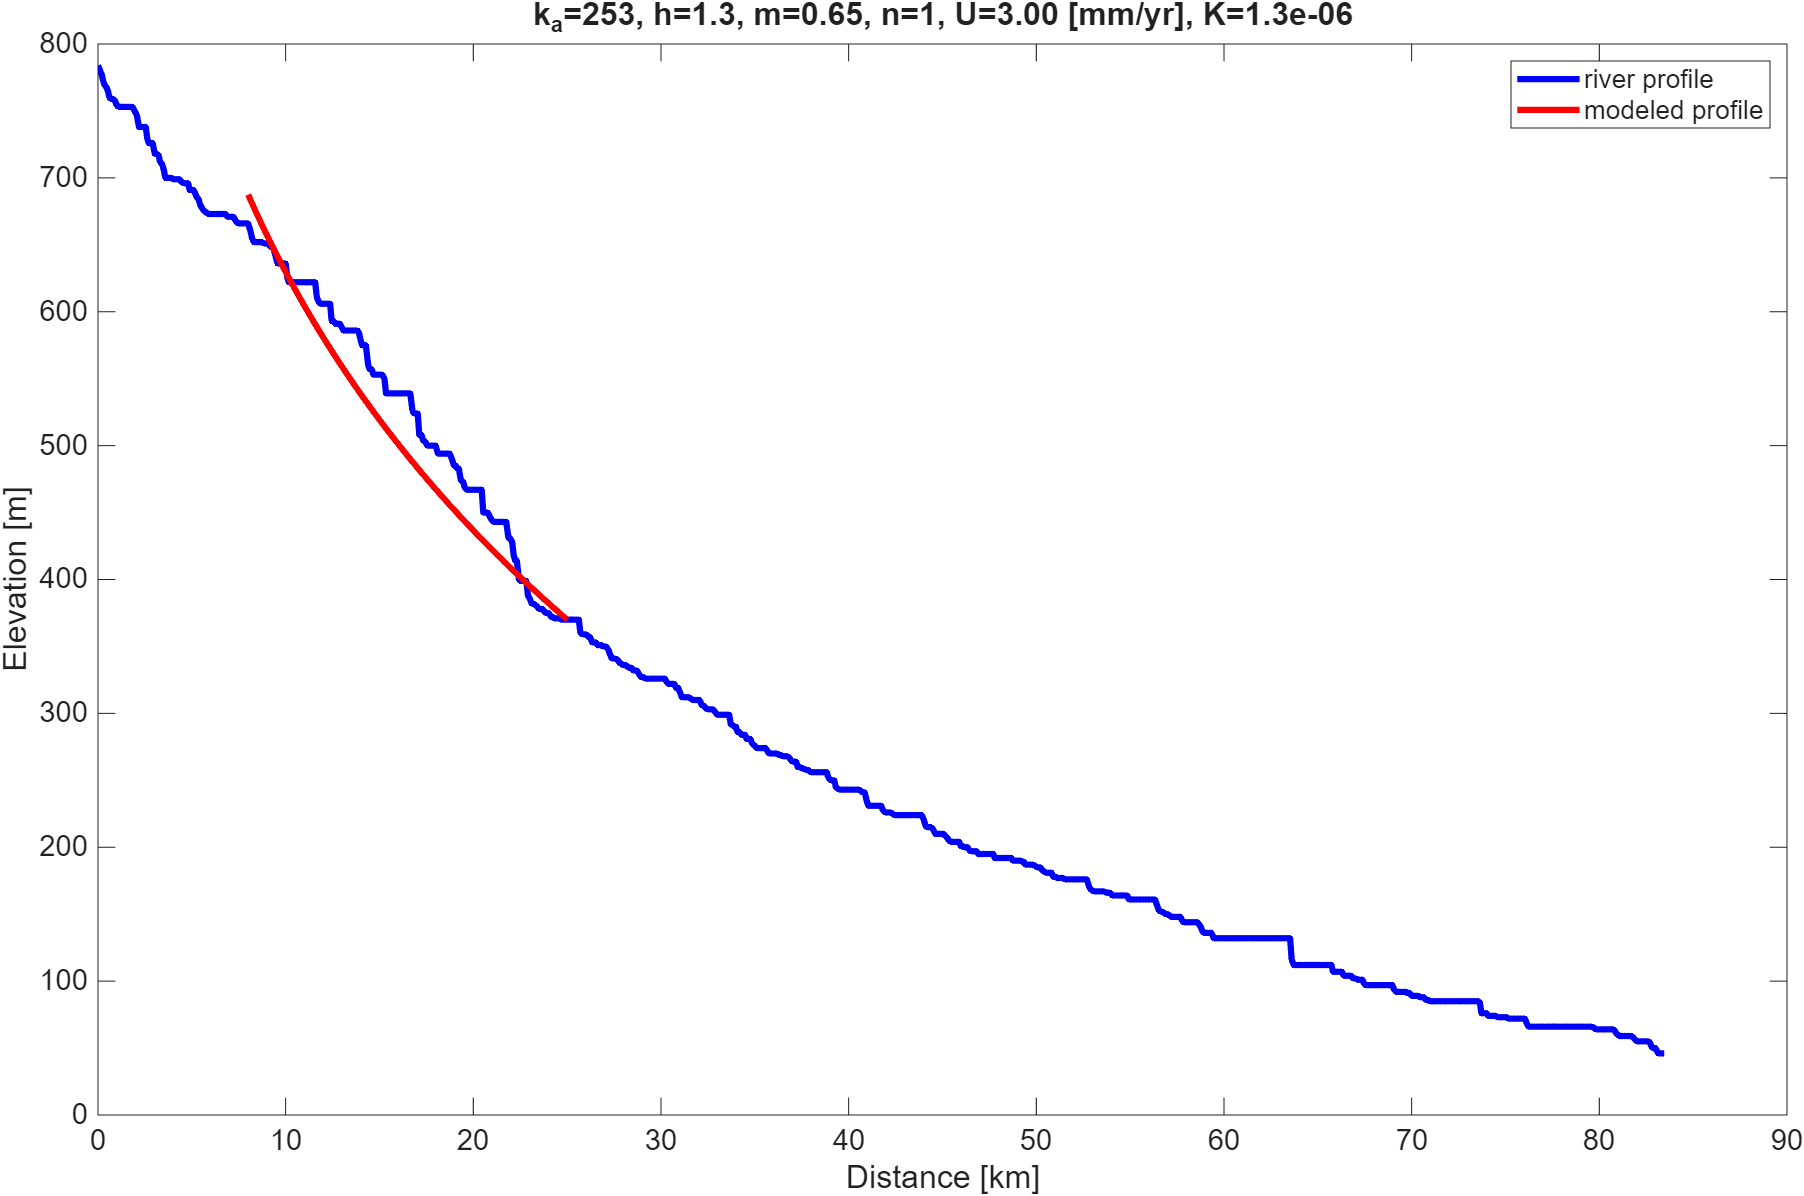
\includegraphics[width=0.8\textwidth]{fit_middle_new.png}
    \caption{Fitted slope gradient, middle section. The fit is poor due to the convex shape
    of the actual profile.}\label{fig:fit_middle}
\end{figure}

\begin{figure}[h]
    \centering
    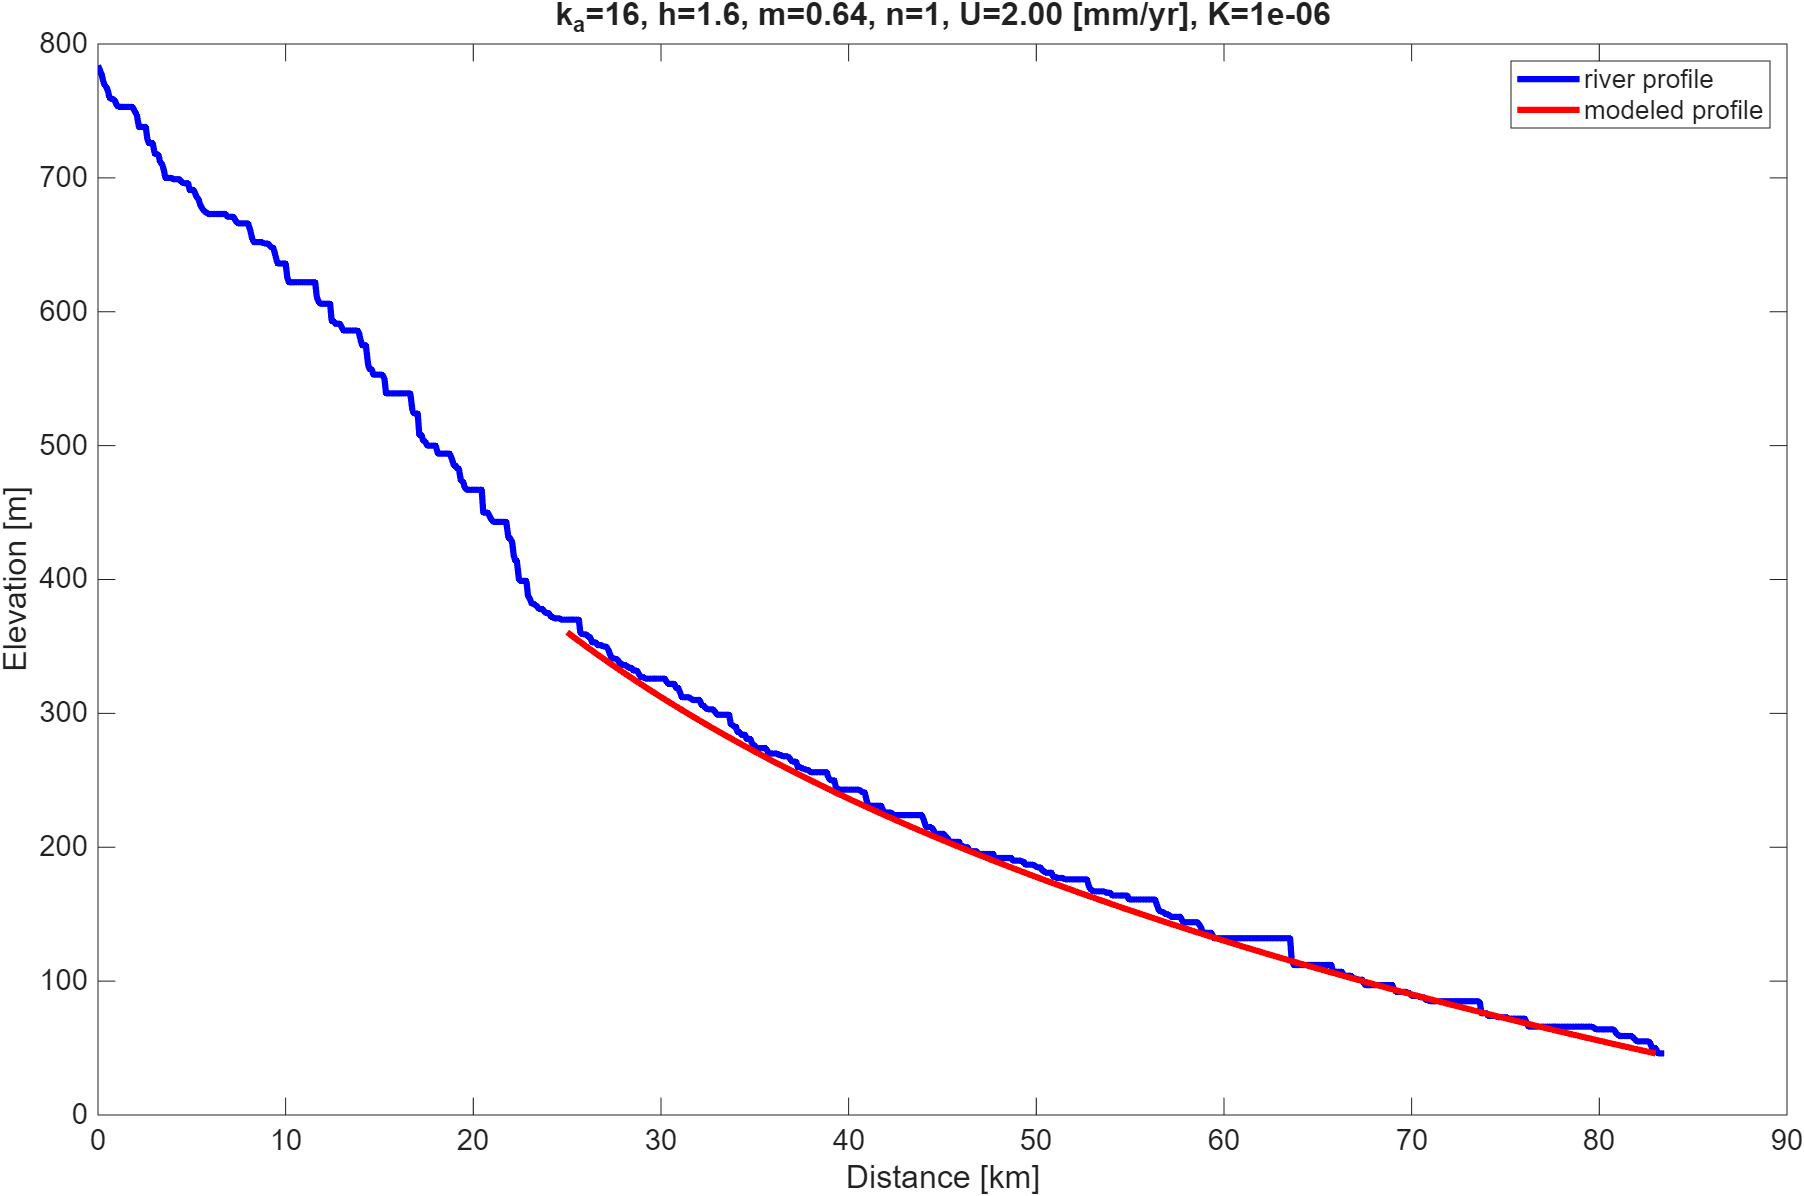
\includegraphics[width=0.8\textwidth]{fit_bottom_new.png}
    \caption{Fitted slope gradient, bottom section.}\label{fig:fit_bottom}
\end{figure}

% Trishear model fits
\begin{figure}[h]
    \centering
    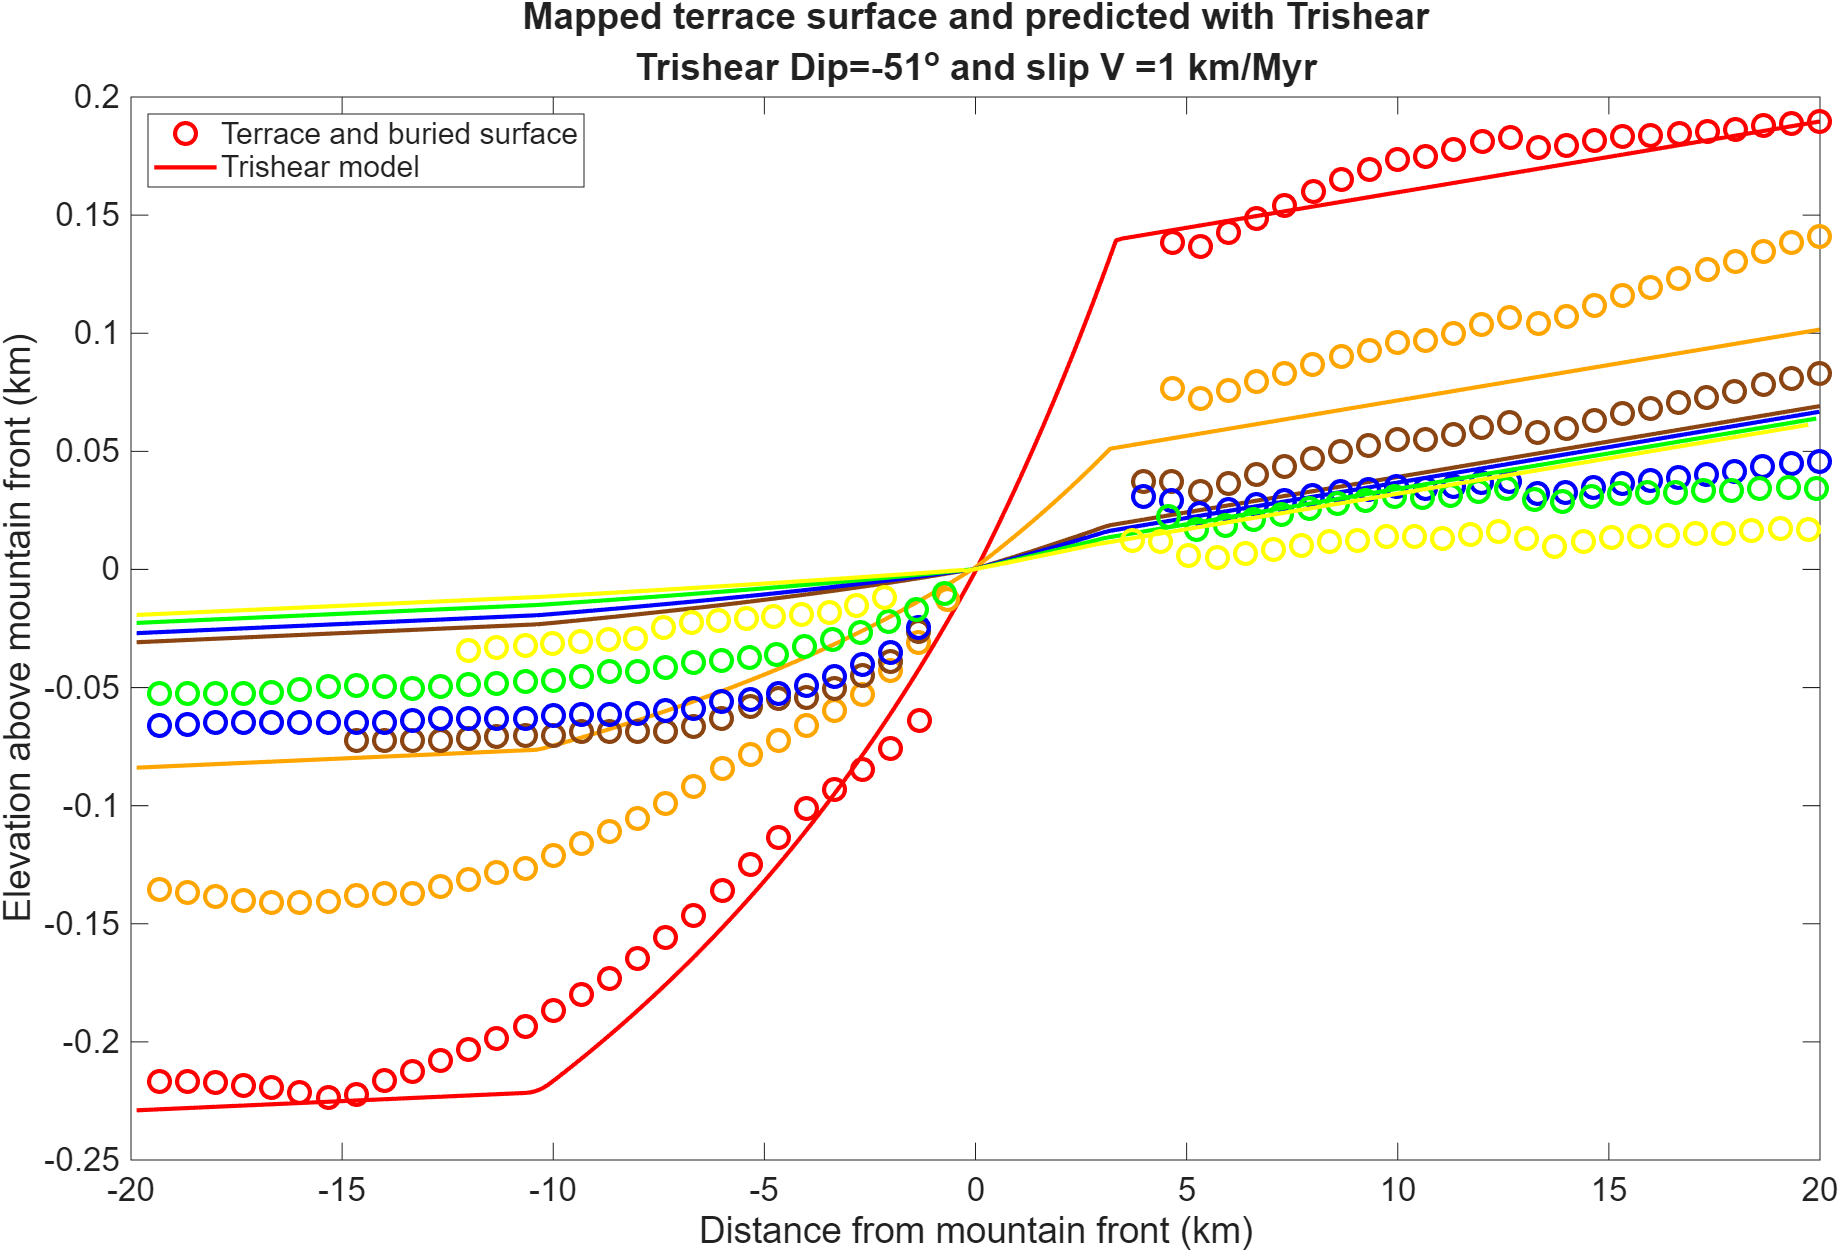
\includegraphics[width=0.8\textwidth]{red_terrace_fit.png}
    \caption{Fitted trishear curve for the \textbf{red} terrace.}\label{fig:fit_red}
\end{figure}

\begin{figure}[h]
    \centering
    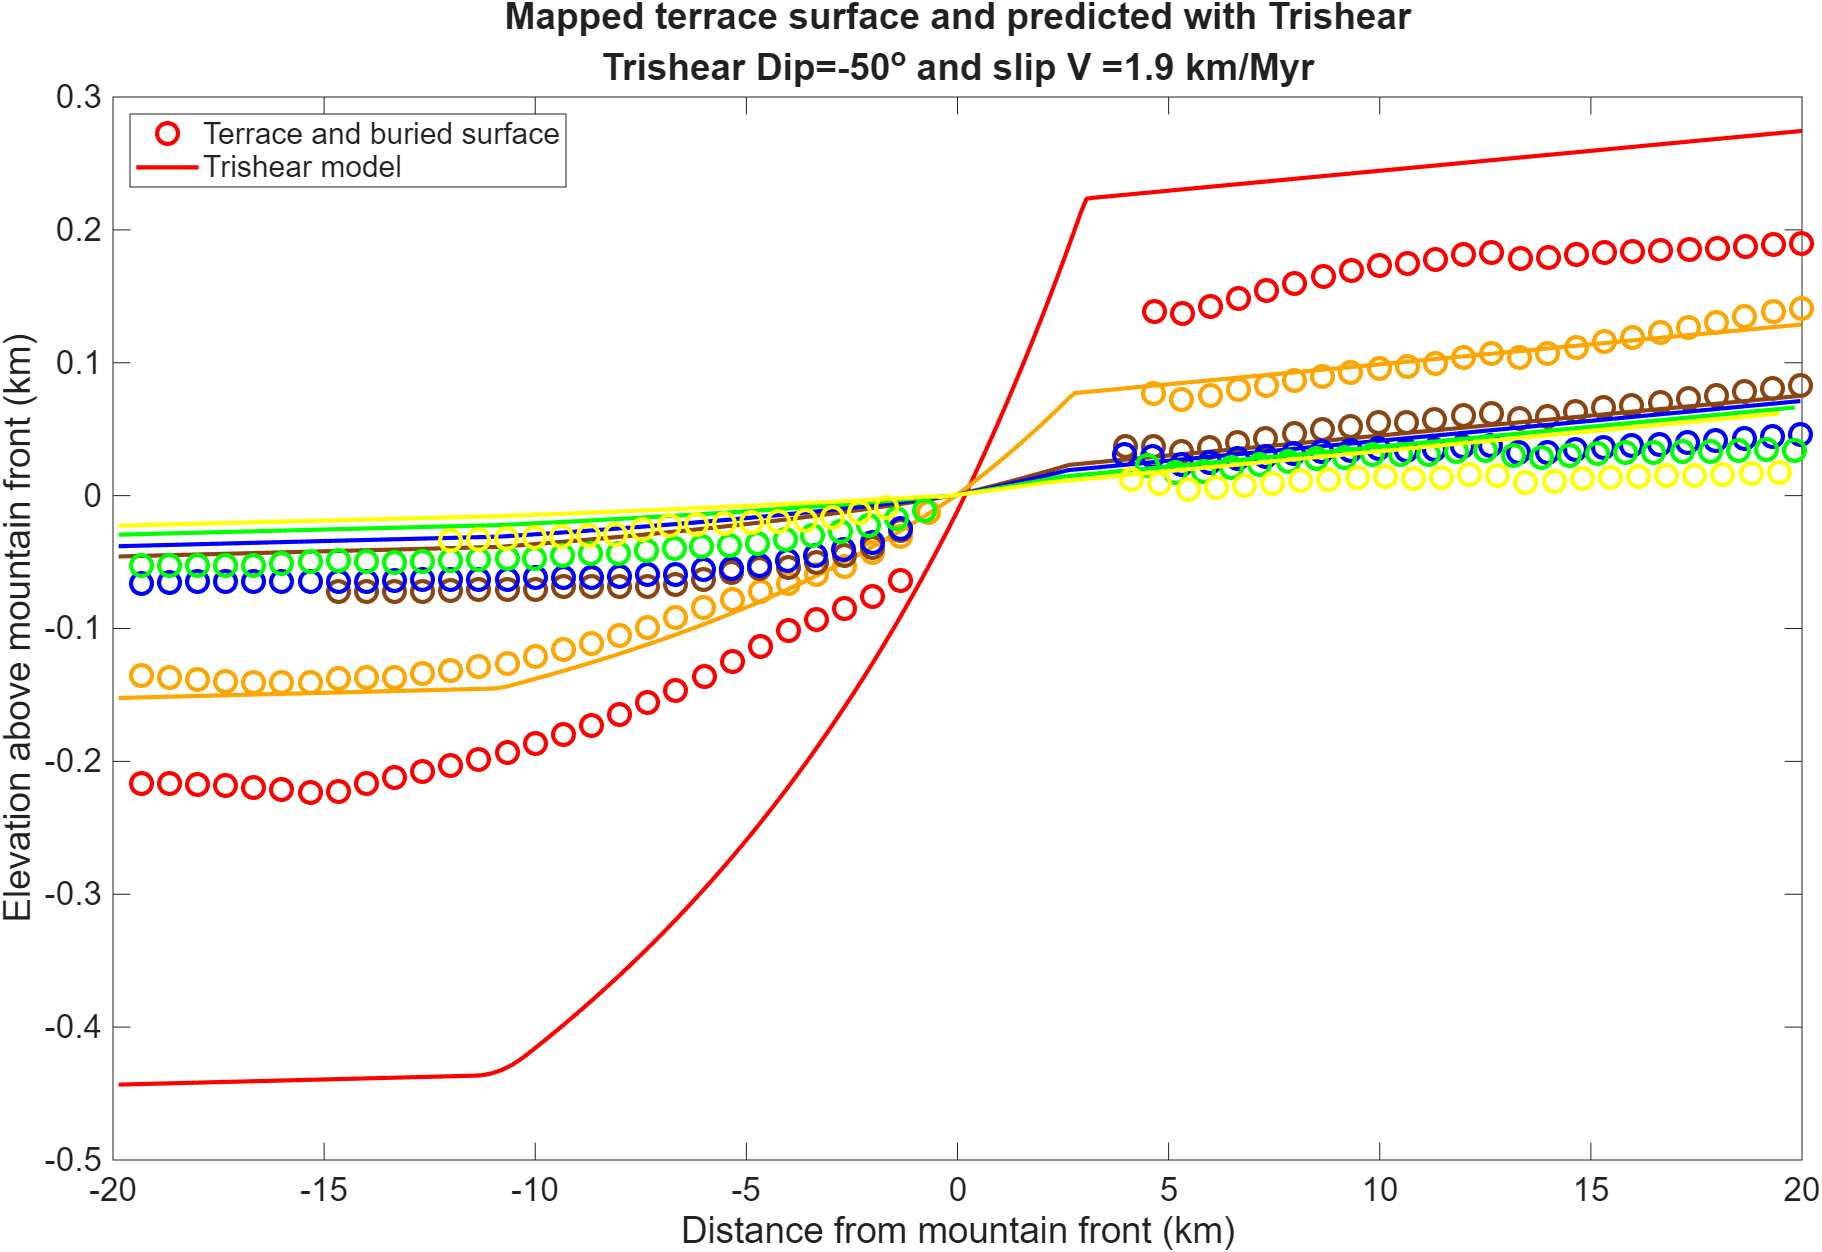
\includegraphics[width=0.8\textwidth]{orange_terrace_fit.png}
    \caption{Fitted trishear curve for the \textbf{orange} terrace.}\label{fig:fit_orange}
\end{figure}

\begin{figure}[h]
    \centering
    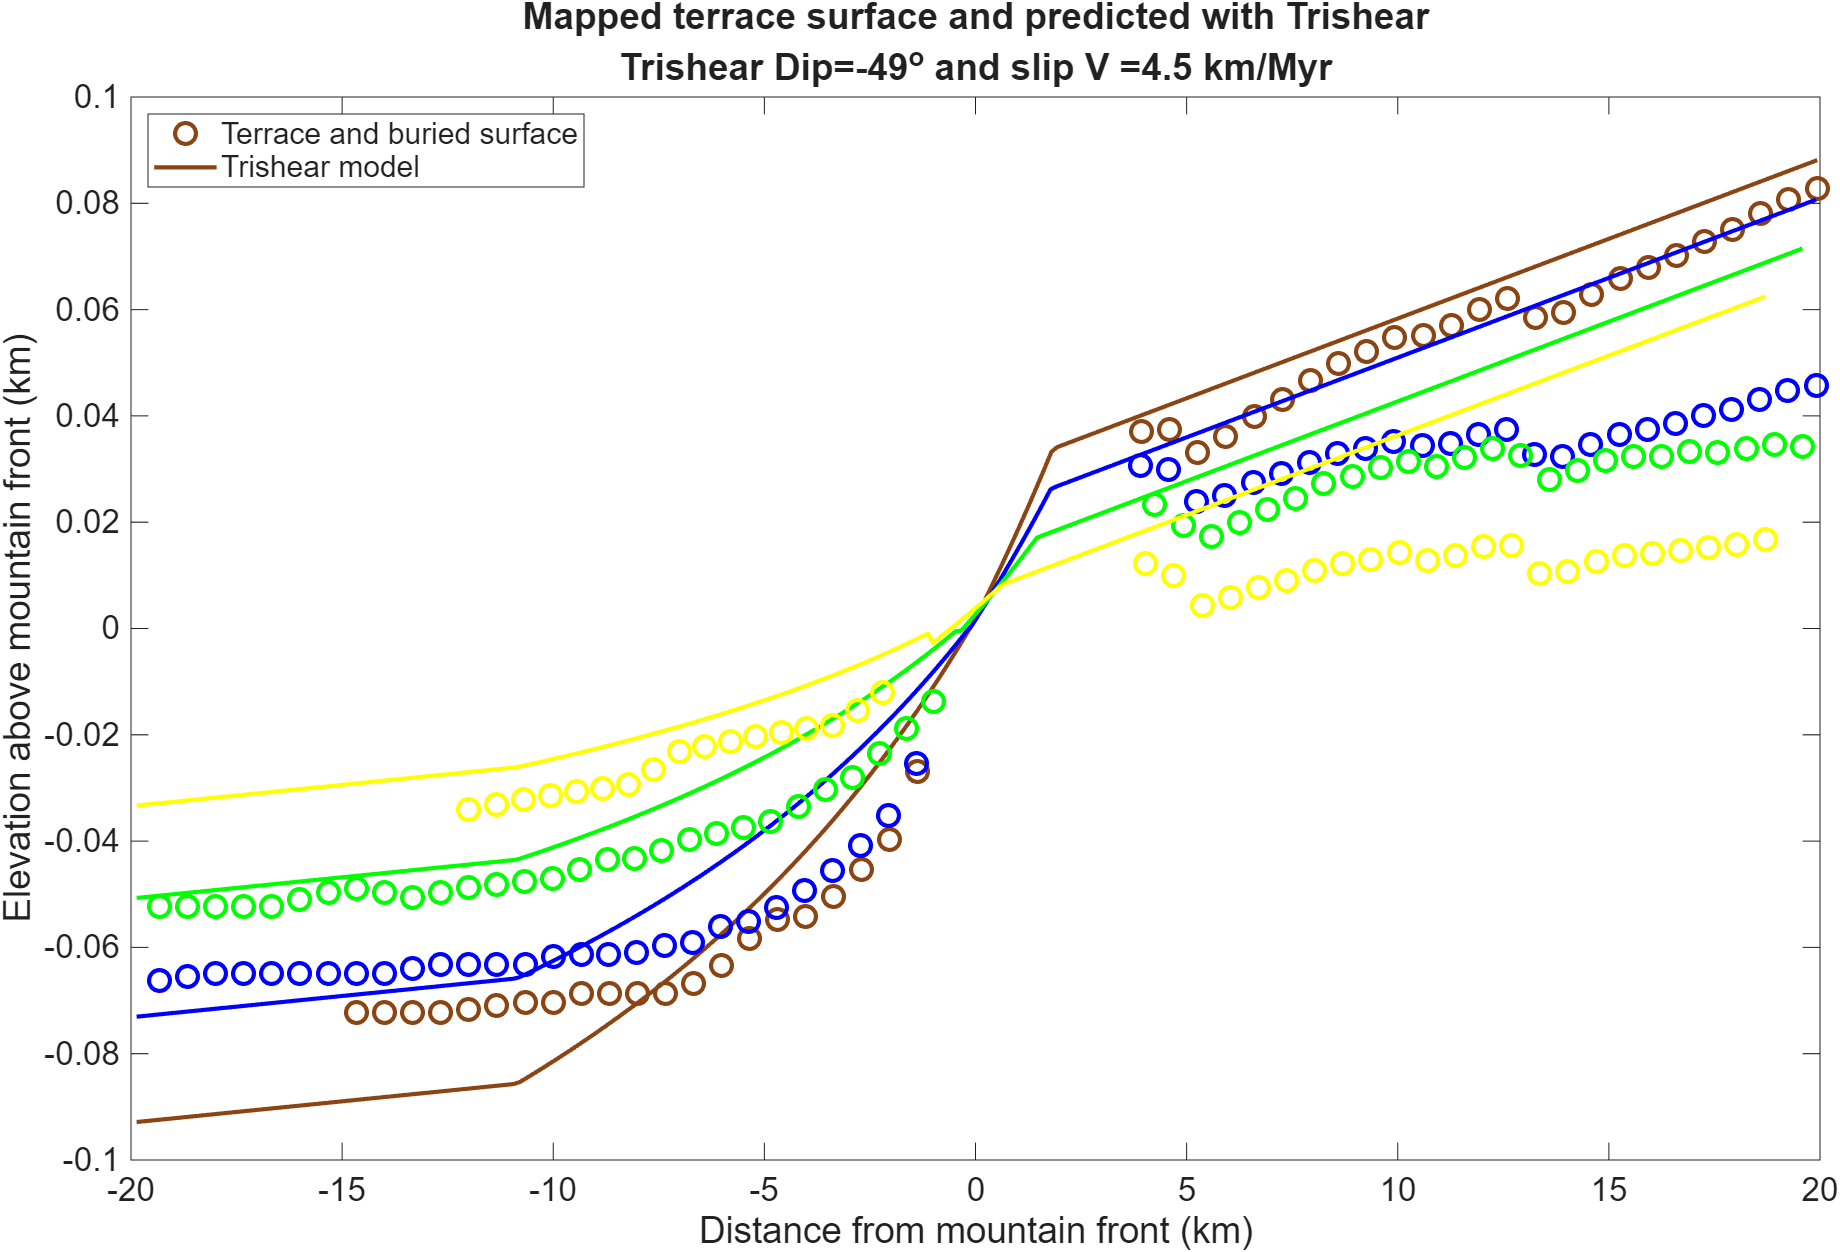
\includegraphics[width=0.8\textwidth]{brown_terrace_fit.png}
    \caption{Fitted trishear curve for the brown terrace. The red and orange terraces are not shown to be
    able to scale the $y$-axis for better visibility of the brown terrace.}\label{fig:fit_brown}
\end{figure}

\end{document}